\section[Прямолинейное движение под действием переменной силы]{Прямолинейное движение под действием переменной силы}

Требуется получить график изменения переменной силы, а также ускорения и координаты тела, на которое эта сила действует.
Сила задана кусочной функцией:

\begin{equation*}
    F(t) = 
    \left\{
        \begin{aligned}
            &3t,\;\; t \leq 5\\
            &0, \;\; 5 < t \leq 10\\
            &-2t, \;\; > 10
        \end{aligned}
    \right. 
\end{equation*}

Получим уравнения и ускорения и координаты тела:
\begin{equation*}
    \begin{aligned}
        &a(t) = \frac{F(t)}{m}\\
        &x(t) = \int a(t)\;dt
    \end{aligned}
\end{equation*}

Моделируем движение тела в Wolfram Mathematicа. 
Используем инструменты: 
\textbf{Piecewise,} 
\textbf{Integrate,} 
\textbf{Plot.}\\[10pt]

\textit{Листинг программы Matematica:}
\begin{lstlisting}
(* Исходные параметры *)
m = 2;
F1[t_] = 3*t;
F2[t_] = 0;
F3[t_] = -2*t;

(* Кусочно заданная функция силы от времени*)
F[t_] = Piecewise[ 
   {
    {F1[t], t <= 5}, 
    {F[5] + F2[t - 5], 5 < t <= 10},
    {F[10] + F3[t - 10], t > 10}
    }, 0
   ];

(* Функции ускорения и координаты от времени *)
a[t_] = F[t] / m;
x[t_] = Integrate[a[t], t];

(* Построение графиков *)
Plot[F[t], {t, 0, 17.5}, AxesLabel -> {t, "F(t)"}]
Plot[a[t], {t, 0, 17.5}, AxesLabel -> {t, "a(t)"}]
Plot[x[t], {t, 0, 17.5}, AxesLabel -> {t, "v(t)"}]
\end{lstlisting} 
\textit{Полученныe графики:}
\begin{figure}[ht]
\centering
    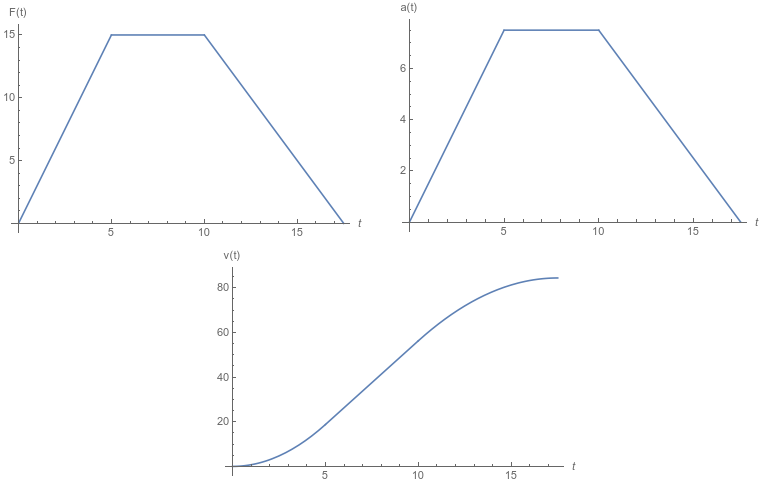
\includegraphics[scale=0.6]{3-rectilinear.png}
\end{figure}
